%tikz_draw
\documentclass[tikz, border=5, svgnames]{standalone}
\usepackage[utf8]{inputenc}
\usepackage[english]{babel}
\usepackage{amsmath}
\usepackage{amsfonts}
\usepackage{amssymb}
%tikzlibrary
\usetikzlibrary{arrows.meta}
%standalone preamble

\usepackage{pgfplots}
\usepackage{ifthen}
\begin{document}

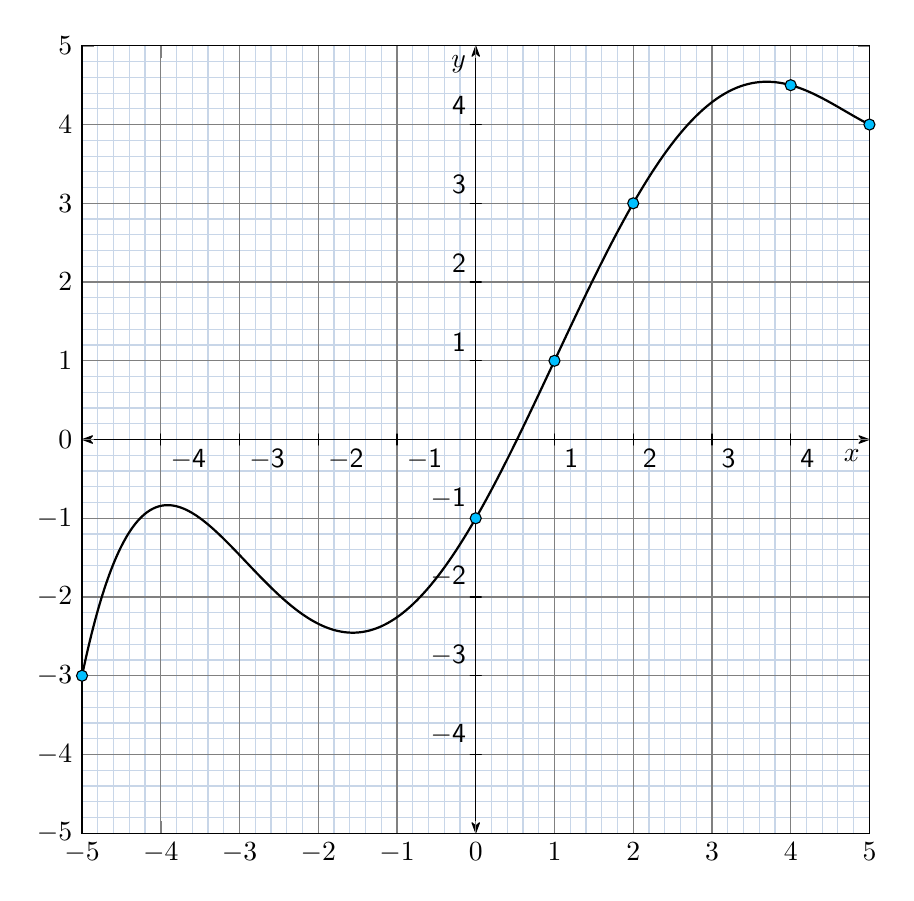
\begin{tikzpicture}

\draw[step=0.2cm,line width=0.4pt,line cap=round,xshift=0cm,yshift=0cm,LightSteelBlue!70!white,opacity=1,solid,] (-5, -5) grid (5, 5);
\draw[step=1cm,line width=0.4pt,line cap=round,xshift=0cm,yshift=0cm,gray,opacity=1,solid,] (-5, -5) grid (5, 5);
\draw (5, 0) node [anchor= north east, ] {$x$};
\draw (0, 5) node [anchor= north east, ] {$y$};

    %axis
    \draw[{Stealth[round]}-{Stealth[round]},,] (-5,0) -- (5,0);
    \draw[{Stealth[round]}-{Stealth[round]},,] (0, -5) -- (0, 5);
	\foreach \x in {-4,...,4}
		\draw[line cap=round,] (\x*1, -2.0pt) -- (\x*1, 2.0pt);
	\foreach \y in {-4,...,4}
		\draw[line cap=round,] (-2.0pt, \y*1) -- (2.0pt, \y*1);
	\foreach \lx in {-4,...,4}
		\draw (\lx*1, 0) node [,anchor=north west,] {$\mathsf{\pgfmathparse{ \lx*1 }\ifthenelse{ \equal{\lx}{0} }{ }{ \pgfmathprintnumber{\pgfmathresult} }}$};
	\foreach \ly in {-4,...,4}
		\draw (0,\ly*1) node [,anchor=south east,] {$\mathsf{\pgfmathparse{ \ly*1 }\ifthenelse{ \equal{\ly}{0} }{ }{ \pgfmathprintnumber{\pgfmathresult} }}$};

\begin{axis}[xmin=-5, xmax=5,ymin=-5, ymax=5, xshift=-5cm, yshift=-5cm, x=1cm,  y=1cm]
\addplot [thick, line cap=round, samples=500, domain=-5:5] {0.00281746031746032*x^5 - 0.0129761904761905*x^4 - 0.111944444444445*x^3 + 0.384404761904762*x^2 + 1.73769841269841*x - 1};
\end{axis}
\filldraw[line width=0.4pt, fill=DeepSkyBlue, draw=Black,opacity=1,] (1,1) circle (2pt);
\filldraw[line width=0.4pt, fill=DeepSkyBlue, draw=Black,opacity=1,] (2,3) circle (2pt);
\filldraw[line width=0.4pt, fill=DeepSkyBlue, draw=Black,opacity=1,] (0,-1) circle (2pt);
\filldraw[line width=0.4pt, fill=DeepSkyBlue, draw=Black,opacity=1,] (5,4) circle (2pt);
\filldraw[line width=0.4pt, fill=DeepSkyBlue, draw=Black,opacity=1,] (-5,-3) circle (2pt);
\filldraw[line width=0.4pt, fill=DeepSkyBlue, draw=Black,opacity=1,] (4.0,4.5) circle (2pt);
\end{tikzpicture}
\end{document}
